\documentclass[11pt,a4paper]{article}

\usepackage{../../templates/style}
\usepackage{subcaption}

\begin{document}

\begin{problem}{Reversi}{standard input}{standard output}{1 second}{64 megabytes}

\textbf{ริเวอสิ (\textit{Reversi} หรือ \textit{Othello})} เป็นเกมที่เล่นกระดานขนาด $8\times 8$ ช่อง ที่เล่นโดยผู้เล่นสองคน โดยคนหนึ่งจะใช้หมากสีดำและอีกคนจะใช้หมากสีขาว 

\begin{figure}[h]
\begin{subfigure}{30ex}
\centering
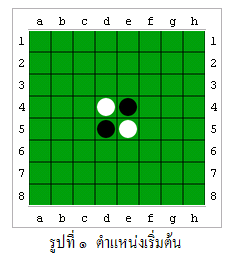
\includegraphics[width=25ex]{../latex/img/1034/1034-1.png}
\end{subfigure}%
\begin{subfigure}{30ex}
\centering
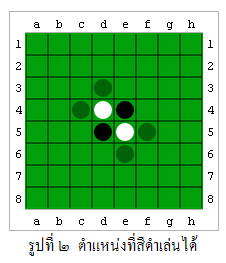
\includegraphics[width=25ex]{../latex/img/1034/1034-2.png}
\end{subfigure}%
\begin{subfigure}{30ex}
\centering
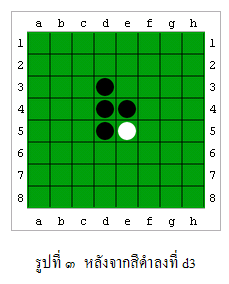
\includegraphics[width=25ex]{../latex/img/1034/1034-3.png}
\end{subfigure}%
\end{figure}
\begin{figure}[h]
\begin{subfigure}{30ex}
\centering
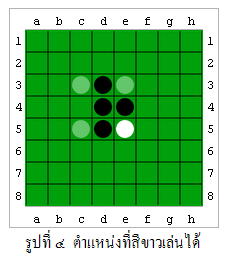
\includegraphics[width=25ex]{../latex/img/1034/1034-4.png}
\end{subfigure}%
\begin{subfigure}{30ex}
\centering
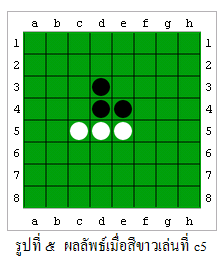
\includegraphics[width=25ex]{../latex/img/1034/1034-5.png}
\end{subfigure}%
\begin{subfigure}{30ex}
\centering
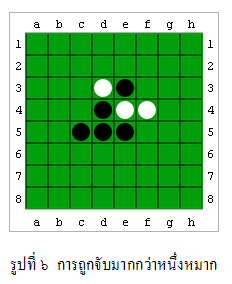
\includegraphics[width=25ex]{../latex/img/1034/1034-6.png}
\end{subfigure}%
\end{figure}

การเริ่มการเล่นทุกครั้งจะต้องวางหมากสีดำและหมากสีขาวอย่างละสองตัวตรงกลางตารางดัง\textit{รูปที่ 1}

ผู้เล่นที่ใช้หมากสีดำจะเป็นผู้เริ่มเล่นก่อนเสมอ โดยการเล่นจะต้องวางหมากลงในตำแหน่งที่มีหมากสีขาวอยู่ตรงกลาง ในแนวนอน แนวตั้ง หรือแนวทะแยงทั้งสองด้าน ซึ่งใน\textit{รูปที่ ๒} เป็นตำแหน่งที่สีดำสามารถจะวางหมากของตัวเองลงได้

ใน\textit{รูปที่ ๓} เป็นผลลัพธ์จากการวางหมากที่ตำแหน่ง $d3$ ซึ่งทำให้หมากสีขาวที่ตำแหน่ง $d4$ "ถูกจับ" ซึ่งทำให้หมากสีขาวที่ $d4$ ถูกเปลี่ยนมาเป็นหมากสีดำ

ทีนี้หมากสีขาวจะเหลือเพียงตัวเดียว \textit{รูปที่ ๔}แสดงตำแหน่งที่วางได้ของสีขาว นั่นก็คือจะต้องมีหมากสีดำอย่างน้อยหนึ่งตัวถูกจับในการวางหมากสีขาวครั้งนี้

ใน\textit{รูปที่ ๕} เป็นการแสดงผลลัพธ์หลังจากที่หมากสีขาวถูกวางหมากที่ $c5$

นอกจากนี้ ในการวางหมากแต่ละครั้งนั้นอาจทำให้หมากของผู้เล่นฝ่ายตรงข้ามถูกจับได้มากกว่าหนึ่งหมาก หากหมากเหล่านั้นถูกปิดหัวท้าย (ในแนวนอน แนวตั้ง และแนวทแยง) ด้วยหมากสีตรงข้ามกับหมากใหม่ที่ถูกวางลงไป เช่นใน\textit{รูปที่ ๖}การวางหมากสีขาวในตำแหน่ง $d6$ จะทำให้หมากสีดำในตำแหน่ง $d4$ $d5$ และ $e5$ ถูกเปลี่ยนเป็นสีขาวทั้งหมด

ผู้เล่นก็จะต้องผลัดกันเล่นอย่างนี้ไปเรื่อยๆ ทั้งนี้จะไม่มีผู้เล่นคนใดลงผิดกติกา ถ้าผู้เล่นคนใดไม่สามารถหาที่วางอย่างถูกกติกาได้กะจะผ่านไปให้ผู้เล่นอีกคนเล่นแทน เมื่อจบเกมผู้เล่นที่มีหมากสีของตัวเองมากกว่าจะเป็นผู้ชนะ



\bigskip
\underline{\textbf{โจทย์}}  จงเขียนโปรแกรมเพื่อรับขั้นตอนการเล่นริเวอสิของผู้เล่นสองคน โดยสีดำเป็นผู้เริ่มเล่นก่อนเสมอ แล้วหาว่าเมื่อวางหมากหมดแล้วตำแหน่งของหมากบนตารางเป็นอย่างไร ทั้งนี้ในข้อมูลทดสอบทุกชุดจะรับประกันว่าการวางทุกครั้งจะมีการวางที่ถูกกติกาเสมอ

\InputFile

\textbf{บรรทัดแรก} รับค่าจำนวนเต็ม $k$ แทนจำนวนหมากทั้งสองสีที่วางในเกมนี้ $(1 \leq k \leq 60)$

\textbf{บรรทัดที่ $2$ ถึง $k+1$} ในบรรทัดที่ $2i$ เป็นข้อมูลการวางหมากครั้งที่ $i$ ของหมากดำ และในบรรทัดที่ $2i+1$ เป็นข้อมูลการวางหมากครั้งที่ $i$ ของหมากขาว โดยแต่ละบรรทัดจะเป็นตำแหน่งบนกระดานที่จะเอาหมากไปวาง ประกอบด้วยตัวอักษรหนึ่งตัว\textbf{ ('a'..'h')} และจำนวนเต็มหนึ่งค่า ($1-8$) คั่นด้วยช่องว่าง

\OutputFile

\textbf{มีแปดบรรทัด} ให้แสดงสถานะของตาราง โดยแต่ละบรรทัดที่ $i$ จะแทนข้อมูลแถวที่ $i$ และแต่ละบรรทัดจะมีตัวอักขระ $8$ ตัวแทนสถานะของแถวนั้น โดยตัวอักขระตัวที่ $1-8$ คือข้อมูลของคอลัมน์ \textbf{a-h} ในแต่ละคอลัมน์จะแทนด้วย
\begin{itemize}

\item \textbf{'.'} (จุดทศนิยม) ถ้าไม่มีหมากใดในช่อง
\item '\textbf{X}' (ตัวอักษรเอ็กซ์ ตัวพิมพ์ใหญ่)ถ้ามีหมากสีดำอยู่ในช่อง และ
\item '\textbf{O}' (ตัวอักษรโอ ตัวพิมพ์ใหญ่) ถ้ามีหมากสีขาวในช่องนั้น
\end{itemize}

\Examples

\begin{example}
\exmp{2
d 3
c 5}{........
........
...X....
...XX...
..OOO...
........
........
........
}%
\end{example}


\Source

การสอบแข่งขันคณิตศาสตร์และวิทยาศาสตร์โอลิมปิกแห่งประเทศไทย
ประจำปี พ.ศ.2549 (สอบแข่งขันรอบที่ 2 ภาคปฏิบัติวันที่ 2)

\end{problem}

\end{document}